% Options for packages loaded elsewhere
\PassOptionsToPackage{unicode}{hyperref}
\PassOptionsToPackage{hyphens}{url}
%
\documentclass[
]{article}
\usepackage{amsmath,amssymb}
\usepackage{iftex}
\ifPDFTeX
  \usepackage[T1]{fontenc}
  \usepackage[utf8]{inputenc}
  \usepackage{textcomp} % provide euro and other symbols
\else % if luatex or xetex
  \usepackage{unicode-math} % this also loads fontspec
  \defaultfontfeatures{Scale=MatchLowercase}
  \defaultfontfeatures[\rmfamily]{Ligatures=TeX,Scale=1}
\fi
\usepackage{lmodern}
\ifPDFTeX\else
  % xetex/luatex font selection
\fi
% Use upquote if available, for straight quotes in verbatim environments
\IfFileExists{upquote.sty}{\usepackage{upquote}}{}
\IfFileExists{microtype.sty}{% use microtype if available
  \usepackage[]{microtype}
  \UseMicrotypeSet[protrusion]{basicmath} % disable protrusion for tt fonts
}{}
\makeatletter
\@ifundefined{KOMAClassName}{% if non-KOMA class
  \IfFileExists{parskip.sty}{%
    \usepackage{parskip}
  }{% else
    \setlength{\parindent}{0pt}
    \setlength{\parskip}{6pt plus 2pt minus 1pt}}
}{% if KOMA class
  \KOMAoptions{parskip=half}}
\makeatother
\usepackage{xcolor}
\usepackage[margin=1in]{geometry}
\usepackage{longtable,booktabs,array}
\usepackage{calc} % for calculating minipage widths
% Correct order of tables after \paragraph or \subparagraph
\usepackage{etoolbox}
\makeatletter
\patchcmd\longtable{\par}{\if@noskipsec\mbox{}\fi\par}{}{}
\makeatother
% Allow footnotes in longtable head/foot
\IfFileExists{footnotehyper.sty}{\usepackage{footnotehyper}}{\usepackage{footnote}}
\makesavenoteenv{longtable}
\usepackage{graphicx}
\makeatletter
\def\maxwidth{\ifdim\Gin@nat@width>\linewidth\linewidth\else\Gin@nat@width\fi}
\def\maxheight{\ifdim\Gin@nat@height>\textheight\textheight\else\Gin@nat@height\fi}
\makeatother
% Scale images if necessary, so that they will not overflow the page
% margins by default, and it is still possible to overwrite the defaults
% using explicit options in \includegraphics[width, height, ...]{}
\setkeys{Gin}{width=\maxwidth,height=\maxheight,keepaspectratio}
% Set default figure placement to htbp
\makeatletter
\def\fps@figure{htbp}
\makeatother
\setlength{\emergencystretch}{3em} % prevent overfull lines
\providecommand{\tightlist}{%
  \setlength{\itemsep}{0pt}\setlength{\parskip}{0pt}}
\setcounter{secnumdepth}{-\maxdimen} % remove section numbering
% definitions for citeproc citations
\NewDocumentCommand\citeproctext{}{}
\NewDocumentCommand\citeproc{mm}{%
  \begingroup\def\citeproctext{#2}\cite{#1}\endgroup}
\makeatletter
 % allow citations to break across lines
 \let\@cite@ofmt\@firstofone
 % avoid brackets around text for \cite:
 \def\@biblabel#1{}
 \def\@cite#1#2{{#1\if@tempswa , #2\fi}}
\makeatother
\newlength{\cslhangindent}
\setlength{\cslhangindent}{1.5em}
\newlength{\csllabelwidth}
\setlength{\csllabelwidth}{3em}
\newenvironment{CSLReferences}[2] % #1 hanging-indent, #2 entry-spacing
 {\begin{list}{}{%
  \setlength{\itemindent}{0pt}
  \setlength{\leftmargin}{0pt}
  \setlength{\parsep}{0pt}
  % turn on hanging indent if param 1 is 1
  \ifodd #1
   \setlength{\leftmargin}{\cslhangindent}
   \setlength{\itemindent}{-1\cslhangindent}
  \fi
  % set entry spacing
  \setlength{\itemsep}{#2\baselineskip}}}
 {\end{list}}
\usepackage{calc}
\newcommand{\CSLBlock}[1]{\hfill\break\parbox[t]{\linewidth}{\strut\ignorespaces#1\strut}}
\newcommand{\CSLLeftMargin}[1]{\parbox[t]{\csllabelwidth}{\strut#1\strut}}
\newcommand{\CSLRightInline}[1]{\parbox[t]{\linewidth - \csllabelwidth}{\strut#1\strut}}
\newcommand{\CSLIndent}[1]{\hspace{\cslhangindent}#1}
\ifLuaTeX
  \usepackage{selnolig}  % disable illegal ligatures
\fi
\usepackage{bookmark}
\IfFileExists{xurl.sty}{\usepackage{xurl}}{} % add URL line breaks if available
\urlstyle{same}
\hypersetup{
  pdftitle={Supplementary materials to TITLE},
  pdfauthor={Martin Papenberg},
  hidelinks,
  pdfcreator={LaTeX via pandoc}}

\title{Supplementary materials to TITLE}
\author{Martin Papenberg}
\date{}

\begin{document}
\maketitle

\subsection{Standard algorithm for
anticlustering}\label{standard-algorithm-for-anticlustering}

To assign samples to batches, we use anticlustering. Anticlustering is
an optimization method that is characterized by (a) an objective
function that quantifies the balance among batches, and (b) an algorithm
that conducts the batch assignment in such a way that balance among
batches is maximized via the objective function. Anticlustering owes its
name to the fact that the objective functions it uses are the reversal
of criteria used in cluster analysis. For example, Späth (1986) already
recognized that by maximizing instead of minimizing the k-means
criterion (the ``variance''), he was able to create groups that are
similar to each other, and presented it as an improvement over the more
intuitive random assignment.

In our application, we optimize the (a) diversity objective using (b)
the exchange algorithm by Papenberg and Klau (2021). This constellation
of objective and algorithm is also the default method implemented in the
R package \texttt{anticlust} (Papenberg 2019). The diversity is defined
as the total sum the within-cluster sums of dissimilarities (Brusco,
Cradit, and Steinley 2020). When assigning samples in such a way that
the diversity is maximized, we simultaneously maximize similarity
between batches. In Papenberg and Klau (2021), we referred to the
maximization of the diversity as ``anticluster editing'' because the
minimization of the diversity is also well-known from the area of
cluster analysis---under the term ``cluster editing'' (Shamir, Sharan,
and Tsur 2004; Böcker, Briesemeister, and Klau 2011).

The anticlustering exchange algorithm takes as input (1) a distance
matrix, quantifying the pairwise dissimilarity among samples, and (2)
the number of batches \(K\). As measure of dissimilarity, we use the
common Euclidean distance, which transfers the features of our samples
to pairwise distances. It is defined as

\[
d(x, y) =  \sqrt{\sum\limits_{i = 1}^{M}(x_i - y_i)^2}
\]

where \(M\) is the number of numeric features describing two samples
\(x\) = (\(x_1, \ldots, x_M\)) and \(y\) = (\(y_1, \ldots, y_M\)). When
samples are described by two features, the Euclidean distance
corresponds to the geometric, ``straightline'' distance between two
points in a two-dimensional space; more similar data points are closer
to each other. Figure~1 illustrates the computation of the Euclidean
distance and the diversity for the numeric features BMI and age that
were used in our motivating application. For categorical variables, we
use binary coding before including them in the computation of the
Euclidean distance. Table 1 illustrates binary coding for the feature
race in our data set, which had five unique values: (a) Asian, (b)
White, (c) Native Hawaiian or Other Pacific Islander, (d) Black, (e)
Native American. Such a categorical variable can be recoded into four
binary variables to maintain the information included in the original
variable.

\begin{figure}

{\centering 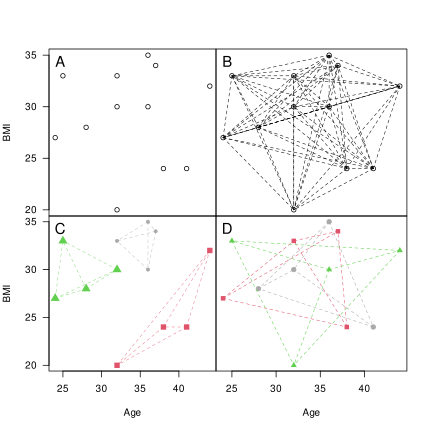
\includegraphics{supplementary_materials_files/figure-latex/unnamed-chunk-2-1} 

}

\caption{Illustrates the conversion from numeric features to Euclidean distance, and (anti)clustering assignments based on minimum and maximum diversity using the Euclidean distance. Panel A illustrates the BMI and age of twelve women in our synthetic data in a scatter plot. Panel B represents the Euclidean distances between features as a straight line in the two-dimensional space. The Euclidean distance is proportional to the length of the connecting lines in panel B. Panel C illustrates a clustering assignment of the 12 data points to $K = 3$ equal-sized groups via \textit{minimum} diversity. Panel D illustrates an anticlustering assignment of the 12 data points to $K = 3$ equal-sized groups via \textit{maximum} diversity. The diversity is computed as the sum of within-(anti)cluster distances, which are highlighted in Panel C and Panel D through connecting lines.}\label{fig:unnamed-chunk-2}
\end{figure}

\begin{longtable}[]{@{}lllll@{}}
\caption{Illustrate the recoding of the variable Race using four binary
variables.}\tabularnewline
\toprule\noalign{}
Race & Black & Native American & Pacific Islander & White \\
\midrule\noalign{}
\endfirsthead
\toprule\noalign{}
Race & Black & Native American & Pacific Islander & White \\
\midrule\noalign{}
\endhead
\bottomrule\noalign{}
\endlastfoot
Black & 1 & 0 & 0 & 0 \\
Pacific Islander & 0 & 0 & 1 & 0 \\
Native American & 0 & 1 & 0 & 0 \\
White & 0 & 0 & 0 & 1 \\
White & 0 & 0 & 0 & 1 \\
Pacific Islander & 0 & 0 & 1 & 0 \\
Pacific Islander & 0 & 0 & 1 & 0 \\
White & 0 & 0 & 0 & 1 \\
Asian & 0 & 0 & 0 & 0 \\
Native American & 0 & 1 & 0 & 0 \\
Native American & 0 & 1 & 0 & 0 \\
Asian & 0 & 0 & 0 & 0 \\
\end{longtable}

The exchange algorithm that maximizes the diversity consists of two
steps: an initialization step and an optimization step. As
initialization, it randomly assigns samples to \(K\) equal-sized
batches. In principle, unequal-sized batches would also be possible with
our algorithm, but equal-sized batches were required in the current
application. After initialization, the algorithm selects the first
sample and checks how the diversity would change if the sample were
swapped with each sample that is currently assigned to a different
batch. After simulating each exchange---that is \(N - \frac{N}{K}\)
exchanges---it realizes the one exchange that increases the diversity
the most. It does not conduct an exchange if no improvement in diversity
is possible. This procedure is repeated for each sample, leading to the
evaluation of \(N \cdot \frac{N}{K}\) exchanges in total; it terminates
after the last sample was processed. The procedure might also restart at
the first element and reiterate through all samples until no exchange
leads to an improvement any more, i.e., until a local maximum is found.
In \texttt{anticlust}, we also implemented this local maximum search,
which corresponds to the algorithm LCW by Weitz and Lakshminarayanan
(1998). For better results, it is also possible to restart the search
algorithm multiple times using different (random) initializations.

\subsection{Including must-link constraints with
anticlustering}\label{including-must-link-constraints-with-anticlustering}

To include must-link constraints with anticlustering, we adjusted both
the initialization phase as well as the optimization phase of the
exchange algorithm. For initialization, we recognize that we now may
have to assign multiple samples simultaneously (``must-link groups'') to
a batch---not all samples can be considered independently of all other
samples. Therefore, we first collect all samples that are have at least
one other sample (``must-link partner'') that has to be assigned to the
same group.

\begin{itemize}
\tightlist
\item
  We obtain a list of all must-link groups together and store them with
  their cardinality.
\item
  We must assign these must-link groups to the \(K\) batches.
\item
  This corresponds to a bin packing problem!

  \begin{itemize}
  \tightlist
  \item
    We have \(n\) elements -- \(n\) = numer of must-link groups -- where
    each element has a size, corresponding to the number of elements in
    that must-link group.
  \item
    Each bin corresponds to a batch and has target capacity of
    \(\frac{N}{K}\)
  \item
    We use ``randomized fit'' heuristic to fill the batches: Select
    first bacthes that fits, and try out batches in random order (leads
    to rather even distribution in all batches). A ``worst fit''
    heuristic might also be used, but some random element is good if we
    restart our optimization heuristic multiple times for better
    results.
  \end{itemize}
\item
  The remaining elements (that are not part of must-link groups) can be
  assigned randomly to batches (while respecting the cardinality
  constraints / equal-sized batches) -- they are not part of the bin
  packing problem.
\end{itemize}

\textbf{Optimization algorithm}:

\begin{itemize}
\tightlist
\item
  ``Merge'' samples: A must-link group is treated as a single unit
  during optimization.
\item
  New distance matrix has to be computed: New distances are given by
  summing up all distances between all elements that are part of
  must-link groups (this works for the diversity objective because it is
  a mere sum)
\item
  Exchange heuristic is conducted on the merged elements. We only
  exchange must-link groups of the same size to ensure that the
  cardinality constraints are still respected in the end (equal-sized
  groups).
\end{itemize}

\subsection*{References}\label{references}
\addcontentsline{toc}{subsection}{References}

\phantomsection\label{refs}
\begin{CSLReferences}{1}{0}
\bibitem[\citeproctext]{ref-bocker2011}
Böcker, Sebastian, Sebastian Briesemeister, and Gunnar W Klau. 2011.
{``Exact Algorithms for Cluster Editing: Evaluation and Experiments.''}
\emph{Algorithmica} 60: 316--34.
\url{https://doi.org/10.1007/s00453-009-9339-7}.

\bibitem[\citeproctext]{ref-brusco2019}
Brusco, Michael J, J Dennis Cradit, and Douglas Steinley. 2020.
{``Combining Diversity and Dispersion Criteria for Anticlustering: A
Bicriterion Approach.''} \emph{British Journal of Mathematical and
Statistical Psychology} 73 (3): 375--96.
\url{https://doi.org/10.1111/bmsp.12186}.

\bibitem[\citeproctext]{ref-R-anticlust}
Papenberg, Martin. 2019. {``Anticlust: Subset Partitioning via
Anticlustering.''} \url{https://cran.r-project.org/package=anticlust}.

\bibitem[\citeproctext]{ref-papenberg2020}
Papenberg, Martin, and Gunnar W Klau. 2021. {``Using Anticlustering to
Partition Data Sets into Equivalent Parts.''} \emph{Psychological
Methods} 26 (2): 161--74. \url{https://doi.org/10.1037/met0000301}.

\bibitem[\citeproctext]{ref-shamir2004vf}
Shamir, Ron, Roded Sharan, and D Tsur. 2004. {``{Cluster graph
modification problems}.''} \emph{Discrete Applied Mathematics} 144:
173--82. \url{https://doi.org/10.1016/j.dam.2004.01.007}.

\bibitem[\citeproctext]{ref-spath1986}
Späth, H. 1986. {``Anticlustering: Maximizing the Variance Criterion.''}
\emph{Control and Cybernetics} 15 (2): 213--18.

\bibitem[\citeproctext]{ref-weitz1998}
Weitz, RR, and S Lakshminarayanan. 1998. {``An Empirical Comparison of
Heuristic Methods for Creating Maximally Diverse Groups.''}
\emph{Journal of the Operational Research Society} 49 (6): 635--46.
\url{https://doi.org/10.1057/palgrave.jors.2600510}.

\end{CSLReferences}

\end{document}
